\chapter{Integralrechnung}
\section{Rekonstruktion einer Größe}
\textit{Beispiel zu...} \\
\textbf{Orientierter Flächeninhalt}\\
Wir betrachten ein Hybridauto, das zunächst 4 Minuten bergab fährt und dabei gleichmäßig abgebremst wird. Anschließend fährt das Auto 2 Minuten bergauf, wobei es gleichmäßig beschleunigt wird. Während des Abbremsens werden der Batterie konstant 0,175 kWh elektrische Energie pro Minute zugeführt. Bei der Fahrt bergauf werden der Batterie konstant 0,32 kWh elektrische Energie pro Minute entnommen. \\

\begin{minipage}{0.5\textwidth}
    Die Abbildung rechts zeigt diesen \\ 
    Energiefluss für die Batterie, \\
    d.h. die Energiezufuhr (positives Vorzeichen) \\
    bzw. die Energieentnahme (neg. Vorzeichen) \\
    pro Zeiteinheit. \\
    
    Die der Batterie zunächst zugeführte \\
    Energie erhalten wir als Produkt der Zeit, in \\
    der das Auto abgebremst wird, mit dem \\
    Energiezufluss in dieser Zeit, also: $$0,175 \ \frac{\text{kWh}}{\text{min}} \cdot 4 \ \text{min} = 0,7$$
\end{minipage}
\begin{minipage}{0.5\textwidth}
    \begin{tikzpicture}[scale=1.25]
        \begin{axis}[clip=true, 
            xmin=-0.5, xmax=7.5, ymin=-3.5, ymax=2.5,
            axis lines = middle, 
            xlabel=Zeit (in min), ylabel=Energiefluss (in kWh pro min),
            xlabel style = {font=\tiny,xshift=0.5ex},
            ylabel style = {font=\tiny,yshift=0.5ex},
            xtick={0,1,...,6,7}, xticklabels={0,1,...,6,7}, yticklabel style = {font=\tiny,xshift=0.5ex},
            xticklabel style = {font=\tiny,yshift=0.5ex},
            ytick={-3,-2,...,1,2}, yticklabels={{-0,3},{-0,2},{-0,1},0,{0,1},{0,2}}]
        \addplot[thick, domain=0:4]{1.75};
        \addplot[thick, domain=4:6]{-3.2};
        \end{axis}
    \end{tikzpicture}
\end{minipage}

Dieses Produkt können wir in der Abbildung durch ein Rechteck über dem Intervall $[0;4]$ oberhalb der Zeit-Achse veranschaulichen.\\
\ \\

Bei der Fahrt bergauf ist der Energiefluss negativ, da der Batterie Energie entnommen wird. Die Energieentnahme erhalten wir nun als $$0,32 \ \frac{\text{kWh}}{\text{min}} \cdot 4 \ \text{min} = 0,64$$
Sie lässt sich durch ein Rechteck über dem Intervall $[4;6]$ unterhalb der Zeit-Achse veranschaulichen. 

Um deutlich zu machen, dass durch den Flächeninhalt des ersten Rechtecks eine Energiezufuhr und durch den Flächeninhalt des zweiten Rechtecks eine Energieentnahme dargestellt wird, versehen wir die Flächeninhalte mit einem negativen bzw. positiven Vorzeichen und sprechen vom \textbf{orientieten Flächeninhalt}
\begin{itemize}
    \item orientierte Flächeninhalt des ersten Rechtecks: $+0,7$ (ohne Maßeinheiten)
    \item orientierte Flächeninhalt des zweiten Rechtecks: $+0,64$ (ohne Maßeinheiten)
\end{itemize}
Somit veranschaulichen die orientierten Flächeninhalte zusammen direkt (bis auf die Einheiten) den gesamten Energiezufluss bzw. -abfluss über den jeweils betrachteten Zeitintervallen. \\
Die Veränderung des Ladezustandes der Batterie über dem gesamten betrachteten Zeitraum erhalten wir dann als Summe der orientierten Flächeninhalte. \\
Hier ist also $0,7 + (-0,64) = 0,06$ die Veränderung des Ladezustandes im Zeitintervall $[0;6]$.

\section{Das Integral als orientierte Flächeninhalt}
\subsection{Das bestimmte Integral nach Riemann}
\begin{minipage}{0.65\textwidth}
    Bei ungleichmäßig beschleunigten Bewegungen ist es schwierig die Fläche unter der Kurve und damit den Weg exakt zu ermitteln. Die Fläche kann aber näherungsweise mithilfe von Rechteckflächen bestimmt werden. Dies kann z. B. wie in der nebenstehenden Abbildung geschehen.\\

    Riemanns Methode besteht darin, sogenannte \textbf{Unter-} und\textbf{ Obersummen} zu bilden (siehe Abbildungen unten). Dazu teilen wir das gewünschte Intervall in gleich große Abschnitte und bilden jeweils die Summe der Flächeninhalte der Rechtecke unterhalb bzw. oberhalb der Kurve.
\end{minipage}
\begin{minipage}{0.35\textwidth}
    $$f(x)=-0,024 \cdot x^2 + 15$$
    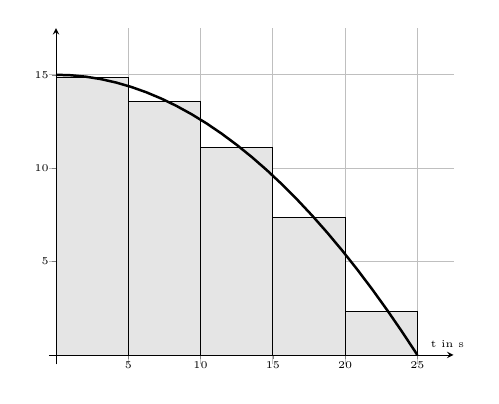
\begin{tikzpicture}[scale=.75]
        \begin{axis}[clip=true, 
            xmin=-0.5, xmax=27.5, ymin=-0.5, ymax=17.5,
            axis lines = middle,
            xlabel=t in s, ylabel=,
            xlabel style = {font=\tiny,xshift=2ex},
            ylabel style = {font=\tiny,yshift=0.5ex},
            xtick={0,5,...,20,25}, xticklabels={0,5,...,20,25}, yticklabel style = {font=\tiny,xshift=0.5ex},
            xticklabel style = {font=\tiny,yshift=0.5ex},
            ytick={0,5,10,15}, yticklabels={0,5,10,15}, grid = major]
            \draw[fill=lightgray!40] (0,0) rectangle (5,14.843);
            \draw[fill=lightgray!40] (5,0) rectangle (10,13.594);
            \draw[fill=lightgray!40] (10,0) rectangle (15,11.094);
            \draw[fill=lightgray!40] (15,0) rectangle (20,7.344);
            \draw[fill=lightgray!40] (20,0) rectangle (25,2.344);
        \addplot[very thick, domain=0:25]{-0.024*x^2 +15};
        \end{axis}
    \end{tikzpicture}
\end{minipage}

\begin{minipage}{0.55\textwidth}
    Der Flächeninhalt A unter der Kurve liegt dann irgendwo dazwischen:
    
    Untersumme < Fläche A < Obersumme.
    
    Je größer die Anzahl n der Teilintervalle ist, desto genauer lässt sich A ermitteln.
    \vspace{-7pt}
    $$\text{Es gilt: }A = \lim_{n\to\infty} U_n = \lim_{n\to\infty} O_n$$
\end{minipage}
\begin{minipage}{0.225\textwidth}
    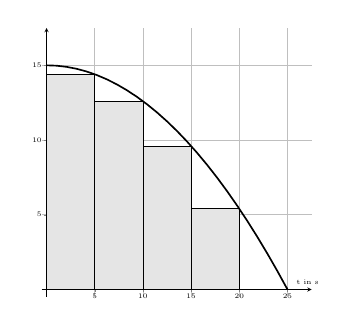
\begin{tikzpicture}[scale=.5]
        \begin{axis}[clip=false, 
            xmin=-0.5, xmax=27.5, ymin=-0.5, ymax=17.5,
            axis lines = middle,
            xlabel=t in s, ylabel=,
            xlabel style = {font=\tiny,xshift=2ex},
            ylabel style = {font=\tiny,yshift=0.5ex},
            xtick={0,5,...,20,25}, xticklabels={0,5,...,20,25}, yticklabel style = {font=\tiny,xshift=0.5ex},
            xticklabel style = {font=\tiny,yshift=0.5ex},
            ytick={0,5,10,15}, yticklabels={0,5,10,15}, y post scale=1.2, grid = major]
            \draw[fill=lightgray!40] (0,0) rectangle (5,14.4);
            \draw[fill=lightgray!40] (5,0) rectangle (10,12.6);
            \draw[fill=lightgray!40] (10,0) rectangle (15,9.6);
            \draw[fill=lightgray!40] (15,0) rectangle (20,5.4);
            \draw[fill=lightgray!40] (20,0) rectangle (25,0);
            \addplot[very thick, domain=0:25]{-0.024*x^2 +15};
        \end{axis}
    \end{tikzpicture}
    \centering Untersumme $U_5$
\end{minipage}
\begin{minipage}{0.225\textwidth}
    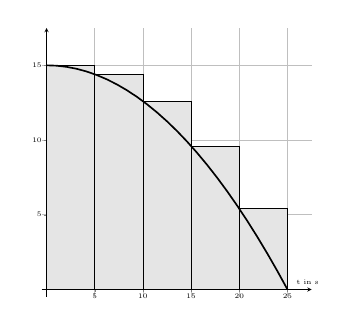
\begin{tikzpicture}[scale=.5]
        \begin{axis}[clip=true, 
            xmin=-0.5, xmax=27.5, ymin=-0.5, ymax=17.5,
            axis lines = middle,
            xlabel=t in s, ylabel=,
            xlabel style = {font=\tiny,xshift=2ex},
            ylabel style = {font=\tiny,yshift=0.5ex},
            xtick={0,5,...,20,25}, xticklabels={0,5,...,20,25}, yticklabel style = {font=\tiny,xshift=0.5ex},
            xticklabel style = {font=\tiny,yshift=0.5ex},
            ytick={0,5,10,15}, yticklabels={0,5,10,15}, y post scale=1.2, grid = major]
            \draw[fill=lightgray!40] (0,0) rectangle (5,15);
            \draw[fill=lightgray!40] (5,0) rectangle (10,14.4);
            \draw[fill=lightgray!40] (10,0) rectangle (15,12.6);
            \draw[fill=lightgray!40] (15,0) rectangle (20,9.6);
            \draw[fill=lightgray!40] (20,0) rectangle (25,5.4);
        \addplot[very thick, domain=0:25]{-0.024*x^2 +15};
        \end{axis}
    \end{tikzpicture}
    \centering Obersumme $O_5$
\end{minipage}

Die auf diese Weise berechnete Fläche nennen wir das \textbf{Riemann-Integral}. \\

\textbf{Merke:}

Die Funktion $f$ sei auf dem Intervall $[a \ ; \ b]$ integrierbar.\\
Die Summe $$\sum^n_{i=1}f(x_i)\cdot h = f(x_1) \cdot h + f(x_2) \cdot h + ... f(x_n) \cdot h + \text{ mit } h = \frac{b - a}{n}$$ sei die \textbf{Zerlegungssumme} von $f$ im Intervall $[a \ ; \ b]$. Der Grenzwert $$\lim_{n \to \infty} S_n = \int_a^bf(x) dx$$ heißt dann das \textbf{bestimmte Integral} der Funktion $f$ in den Grenzen von $a$ bis $b$. \footnote{Diese Zerlegungsfuntionen werden auch Treppenfunktionen genannt.}


\begin{definition}
    Gegeben ist eine Funktion $f$, die auf dem Intervall $[a \ ; \ b]$ integrierbar ist. Das (bestimmte) Integral von $f$ über $[a \ ; \ b]$ ist der orientierte Flächeninhalt, den der Graph von $f$ mit der $x$-Achse zwischen der unteren Grenze $a$ und der oberen Grenze $b$ einschließt.
    
    Wir schreiben hierfür: $$\int_a^bf(x) dx$$
    Hierbei gilt: $$\lim_{n \to \infty} \sum^n_{i = 1}f(x_i) \cdot \Delta x = \int_a^bf(x) dx$$
    \begin{itemize}
        \item Lies: Integral $f(x)$ $dx$ von $a$ bis $b$
        \item $f(x)$ heißt Integrand
        \item $x$ heißt Integrationsvariable
        \item $dx$ gibt die Integrationsvariable an, hierbei steht $d$ für Differential
        \item $a$ heißt untere, $b$ obere Integrationsgrenze
    \end{itemize}
\end{definition}

\section{Bilden von Stammfunktionen}
\textit{Beispiel} \\
Gib eine Funktion an, deren Ableitung eine

\begin{minipage}{0.75\textwidth}
    konstante Funktion, z.B. $f^\prime(x) = 1$, \\
    linerare Funktion, z.B. $f^\prime(x) = x$ bzw. \\
    quadratische Funktion, z.B. $f^\prime(x) = 3x^2$ ist. \\
\end{minipage}
\begin{minipage}{0.25\textwidth}
    $\to \ f(x) = x$ \\
    $\to \ f(x) = \frac{x^2}{2}$ \\
    $\to \ f(x) = x^3$ \\
\end{minipage}

\begin{definition}
    Es sei ein Funktion $f$ gegeben, mit $f(x) = x^n$, so bildet sich die Stammfunktion $F$ folgendermaßen: $$F(x) = \frac{x^{n+1}}{n+1} + C \qquad \footnote{wichtige Ausnahme: $f(x) = \frac{1}{x} \to F(x) = \ln{(|x|)} + C$} $$ 
\end{definition}

\textit{Beispiel: Bestimmen einer speziellen SF (Stammfunktion)} 
\begin{align*}
    f(x) = (x + 2) ^2 \ ; F(0) = 1 \\
    (1) \ F(x) &= \frac{1}{3}(x + 2)^3 + C \\
    (2)\ F(0) &= 1 \\
    1 &= \frac{8}{3} + C \\
    C &= - \frac{5}{3} \quad \quad \Rightarrow F(x) = \frac{1}{3}(x + 2)^3 - \frac{5}{3}
\end{align*}

\subsection{Merkhilfe: Stammfunktionen und Bildungsregeln}

\textbf{Bestimmung von Stammfunktionen}\\
Sind $G$ und $H$ Stammfunktionen von $g$ und $h$, so gelten für die Bildung von Stammfunktionen folgende Regeln:\\
\begin{tabular} { | p{0.2\textwidth} | p{0.2\textwidth} | p{0.2\textwidth} | p{0.2\textwidth} | p{0.2\textwidth} | }
     \hline
       & Potenzregel \linebreak ($n \neq -1$) & Konstanter \linebreak Faktor & Summenregel & Lineare \linebreak Substitution \\
     \hline
     \begin{center} Funktion $f$ mit $f(x) =$ \end{center} & \begin{center} \vspace{5pt}$x^n$ \end{center} & \begin{center} \vspace{5pt}$c \cdot g(x) ; c \in \mathbb{R}$ \end{center} & \begin{center} \vspace{5pt}$g(x) + h(x)$ \end{center}  & \begin{center} \vspace{5pt}$g(m \cdot x + c)$ \end{center} \\
     \hline
     \begin{center} Stammfunktion $F$ mit $F(x) =$ \end{center} & \begin{center} \vspace{5pt}$\frac{1}{n+1}x^{n+1}$ \end{center} & \begin{center} \vspace{5pt}$c \cdot G(x); c \in \mathbb{R}$ \end{center} & \begin{center} \vspace{5pt}$G(x) + H(x)$ \end{center}  & \begin{center} \vspace{5pt}$\frac{1}{m} \cdot G(m \cdot x +c)$ \end{center} \\
    \hline
\end{tabular}
\textbf{Merke:} Die lineare Substitution gilt nur, wenn die innere Funktion eine linere Funktion ist. \\
\textit{Gegenbeispiel:}\\
$f(x) = e^{x^2 + 1}; x \in \mathbb{R}$ \\
Die Funktion $G(x) = \frac{1}{2x} \cdot e^{x^2 + 1}$ ist \textbf{keine Stammkunktion} von $f$, da die Ableitung der Funktion $G$ mithilfe der Quotientenregel sich zu $(G(x))^\prime = \frac{2x \cdot e^{x^2 + 1} \cdot (2x) - e^{x^2 + 1} \cdot 2}{(2x)^2} = e^{x^2 + 1} - \frac{2e^{x^2 + 1}}{4x^2}$ ergibt. Dies ist nicht das Gleiche wie $f(x) = e^{x^2 + 1}$. Somit ist $(G(x))^\prime \neq f(x)$. Daraus folgt, dass $G$ keine Stammfunktion von $f$ ist.

\textbf{\glqq Ableitungskreislauf\grqq \ für Sinus- und Kosinusfunktionen}

\begin{tikzpicture}[node distance=2cm]
    \node (pro1) [process, text width=5cm] {$\sin{(x)}$};
    \node (pro2a) [process, text width=5cm, left of=pro1, xshift = -4cm, yshift= -2cm] {$-\cos{(x)}$};
    \node (pro2b) [process, text width=5cm, right of=pro1, xshift = 4cm, yshift= -2cm] {$\cos{(x)}$};
    \node (pro3) [process, below of=pro1, text width=5cm, yshift= -2cm] {$-\sin{(x)}$};
    
    \begin{scope}[transform canvas={xshift=-0.25em, yshift=0.25em}]
        \draw [arrow, color=red] (pro2a) |- (pro1);
    \end{scope}
    \begin{scope}[transform canvas={xshift=-0.75em, yshift=0.75em}]
        \draw [arrow, color=blue] (pro1) -| (pro2a);
    \end{scope}
    \begin{scope}[transform canvas={xshift=0.25em, yshift=0.25em}]
        \draw [arrow, color=red] (pro1) -| (pro2b);
    \end{scope}
    \begin{scope}[transform canvas={xshift=0.75em, yshift=0.75em}]
        \draw [arrow, color=blue] (pro2b) |- node[above] {Stammfunktion} (pro1);
    \end{scope}
    \begin{scope}[transform canvas={xshift=0.25em, yshift=-0.25em}]
        \draw [arrow, color=red] (pro2b) |- (pro3);
    \end{scope}
    \begin{scope}[transform canvas={xshift=0.75em, yshift=-0.75em}]
        \draw [arrow, color=blue] (pro3) -| (pro2b);
    \end{scope}
    \begin{scope}[transform canvas={xshift=-0.25em, yshift=-0.25em}]
        \draw [arrow, color=red] (pro3) -| node[above right] {Ableitung} (pro2a);
    \end{scope}
    \begin{scope}[transform canvas={xshift=-0.75em, yshift=-0.75em}]
        \draw [arrow, color=blue] (pro2a) |- (pro3);
    \end{scope}
\end{tikzpicture}

\textbf{Ableitung und Stammfunktion zu wichtigen Funktionen}\\
\begin{tabular} { | p{0.087\textwidth} | p{0.087\textwidth} | p{0.087\textwidth} | p{0.087\textwidth} |p{0.087\textwidth} | p{0.087\textwidth} |p{0.087\textwidth} | p{0.087\textwidth} |p{0.087\textwidth} | p{0.087\textwidth} |}
     \hline
     \begin{center} $F(x) =$ \end{center} & \begin{center} $\frac{1}{3}x^3$ \end{center} & \begin{center} $\frac{1}{2}x^2$ \end{center} & \begin{center} $x$ \end{center} & \begin{center}  $\ln{(|x|)}$ \end{center} & \begin{center} $-x^{-1}$ \end{center} &  \vspace{3pt}\centering$x\ln{(x)} -x$  & \begin{center} $e^x$ \end{center} & \begin{center} -$\cos{(x)}$ \end{center} & \begin{center} $\sin{(x)}$  \end{center}  \\
     \hline
     \begin{center} $f(x) =$ \end{center} & \begin{center} $x^2$ \end{center} & \begin{center} $x$ \end{center} & \begin{center} $1$ \end{center} & \begin{center}  $x^{-1}$ \end{center} & \begin{center} $x^{-2}$ \end{center} & \begin{center} $\ln{x}$ \end{center} & \begin{center} $e^x$ \end{center} & \begin{center} $\sin{(x)}$ \end{center} & \begin{center} $\cos{(x)}$  \end{center}  \\
     \hline
     \begin{center} $f^\prime(x) =$ \end{center} & \begin{center} $2x$ \end{center} & \begin{center} $1$ \end{center} & \begin{center} $0$ \end{center} & \begin{center}  $-x^{-2}$ \end{center} & \begin{center} $-2x^{-3}$ \end{center} & \begin{center} $\frac{1}{x}$ \end{center} & \begin{center} $e^x$ \end{center} & \begin{center} $\cos{(x)}$ \end{center} & \begin{center} -$\sin{(x)}$  \end{center}  \\
    \hline
\end{tabular}

\textbf{Hinweis:}\\
Bei allen Stamfunktionen kann beim Funktionsterm ein $+C$ notiert werden. Hierbei ist $C$ eine Konstante.

\section{Der Hauptsatz der Differential- und Integralrechnung (HDI)}

\glqq kurz und knapp:\grqq $$\int_a^bf(x)dx = \left[F(x)\right]^b_a = F(b) - F(a)$$

\textit{Beispiel: Wert des Integrals}
\begin{align*}
    \int_{-3}^{-1}-5dx = \left[-5x\right]_{-3}^{-1} = -5 \cdot (-1) - (-5\cdot(-3)) = 5 - 15 = -10 &&
\end{align*}

\section{Integralfunktion}

\begin{definition}
    Sei $f$ eine Funktion, die im Intervall $I$ integrierbar ist und sei $a \in I$. Die Funktion $J_a$ mit $$J_a(x) = \int_a^xf(t)dt \text{ mit } a \in I$$ heißt \textbf{Integralfunktion von f zur unteren Grenze a}.
\end{definition}

\textbf{Merke:} Eine Integralfunktion hat mindestens eine Nullstelle haben.

\textit{Beispiel:} \\
Die Folgende Funktion $G_a$ soll keine Integralfunktion von g sein: $G_a(x)= 2x^2 -5x + a$\\
Die Werte von a müssen so gewählt werden, dass $G_a$ keine Nullstelle hat.
\begin{align*}
    G_a(x) &= 0 \\
    0 &= 2x^2 -5x + a \\
    x_{1,2} &= \frac{5 \pm \sqrt{25 - 8a}}{4} 
\end{align*}
Wenn $G_a$ keine Nullstelle haben soll, so muss die Diskriminante negativ, also $<0$ sein:
\begin{align*}
    25 - 8a &< 0 \\
    a &> \frac{25}{8}
\end{align*}
Also: $a> \frac{25}{8}$

\section{Stammfunktionen und ihre Graphen}

\textbf{allg. gilt:} $f(x) > 0 \Longleftrightarrow F^\prime(x) > 0$ \\
Damit: F ist streng monoton steigend!

\section{Integral und Flächeninhalt}

offen

